\documentclass[xcolor=svgnames]{beamer}

\usepackage[resetfonts]{cmap}
\usepackage[T1]{fontenc}
\usepackage{lmodern}

\usepackage[utf8]{inputenc}
\usepackage[czech]{babel}

\usepackage{tikz}
\usetikzlibrary{arrows,positioning}

\usepackage{verbatim}
\usepackage{listings}
\usepackage{textcomp}
\usepackage{graphicx}
\usepackage{wasysym}
\usepackage{amsmath}
\usepackage{booktabs}
\usepackage{tikz}
\usepackage{pgf-pie}
\usepackage{calc}
\usepackage{ifthen}


\usetheme{Arteffi}
\def\topic{}


\begin{document}

% --------------------------- SLIDE --------------------------------------------
\title[Obhajoba bakalářské práce]{Automatické generování otázek a~adaptabilní procvičování}
%\{B}
\author{Tomáš Effenberger}
\institute{Masarykova univerzita\\Fakulta informatiky}
\date{\today}
\frame[plain]{\titlepage}
% ------------------------------------------------------------------------------

% --------------------------- SLIDE --------------------------------------------
{
\usebackgroundtemplate{\hspace{-1.6cm}
\includegraphics[scale=0.3]{img/home-page-large.png}}
%\usebackgroundtemplate{%
%\tikz \node[at=(current page.center)] {
%
\includegraphics[scale=0.50]{img/home-page-large.png}};
%}
\begin{frame}[plain]
\end{frame}
}
% ------------------------------------------------------------------------------
% --------------------------- SLIDE --------------------------------------------
{
\usebackgroundtemplate{\hspace{-1.6cm}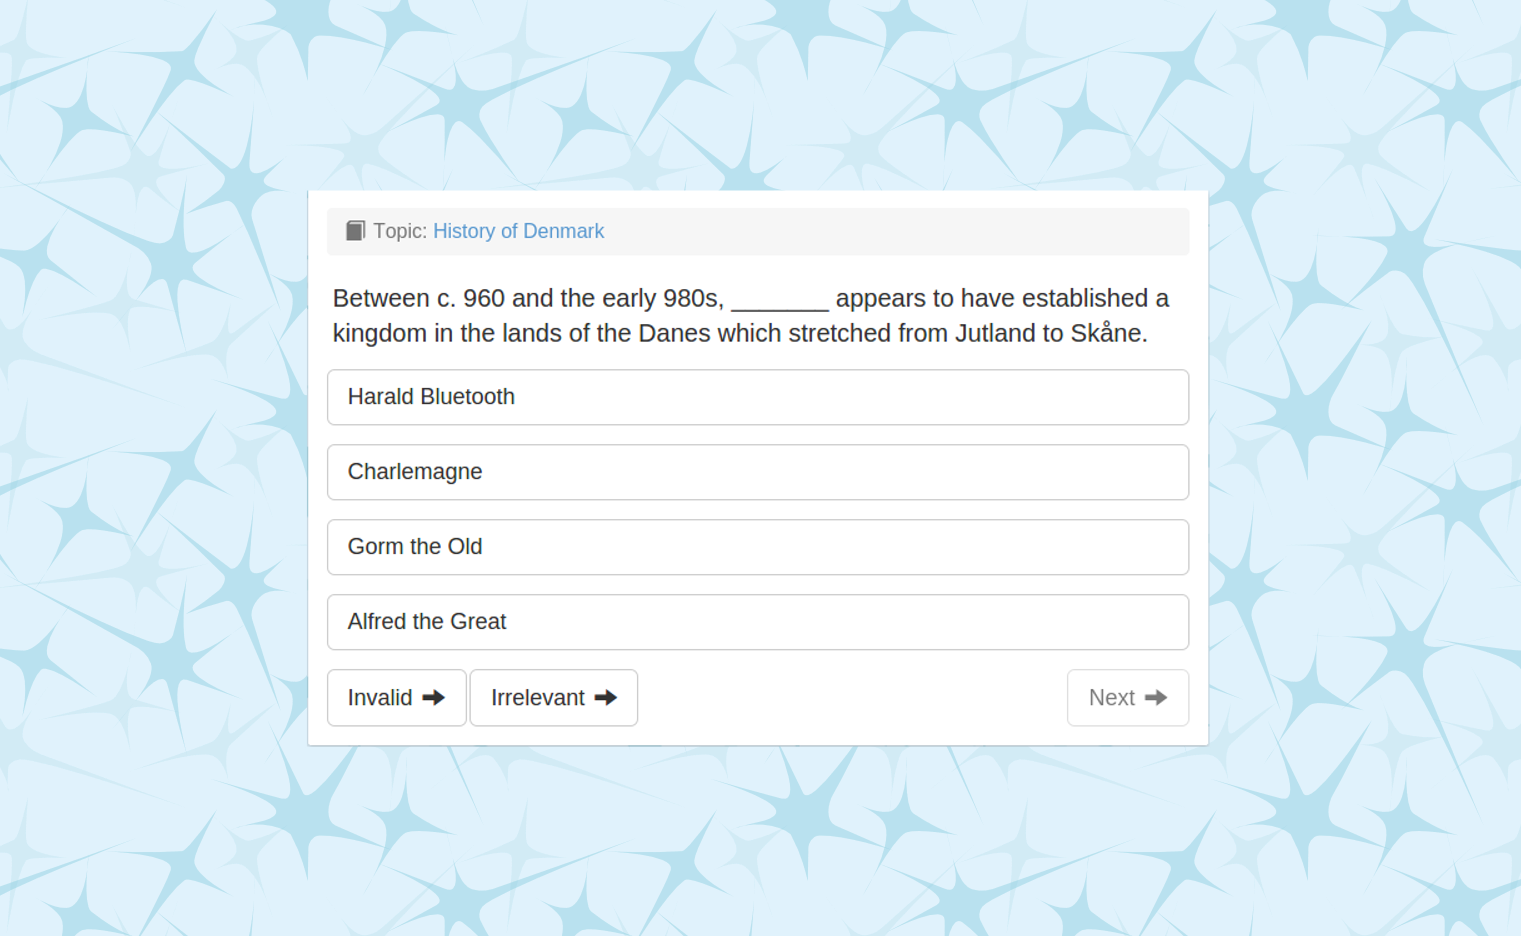
\includegraphics[scale=0.3]{img/question-unanswered2.png}}
\begin{frame}[plain]
\end{frame}
}
% ------------------------------------------------------------------------------
% --------------------------- SLIDE --------------------------------------------
{
\usebackgroundtemplate{\hspace{-1.6cm}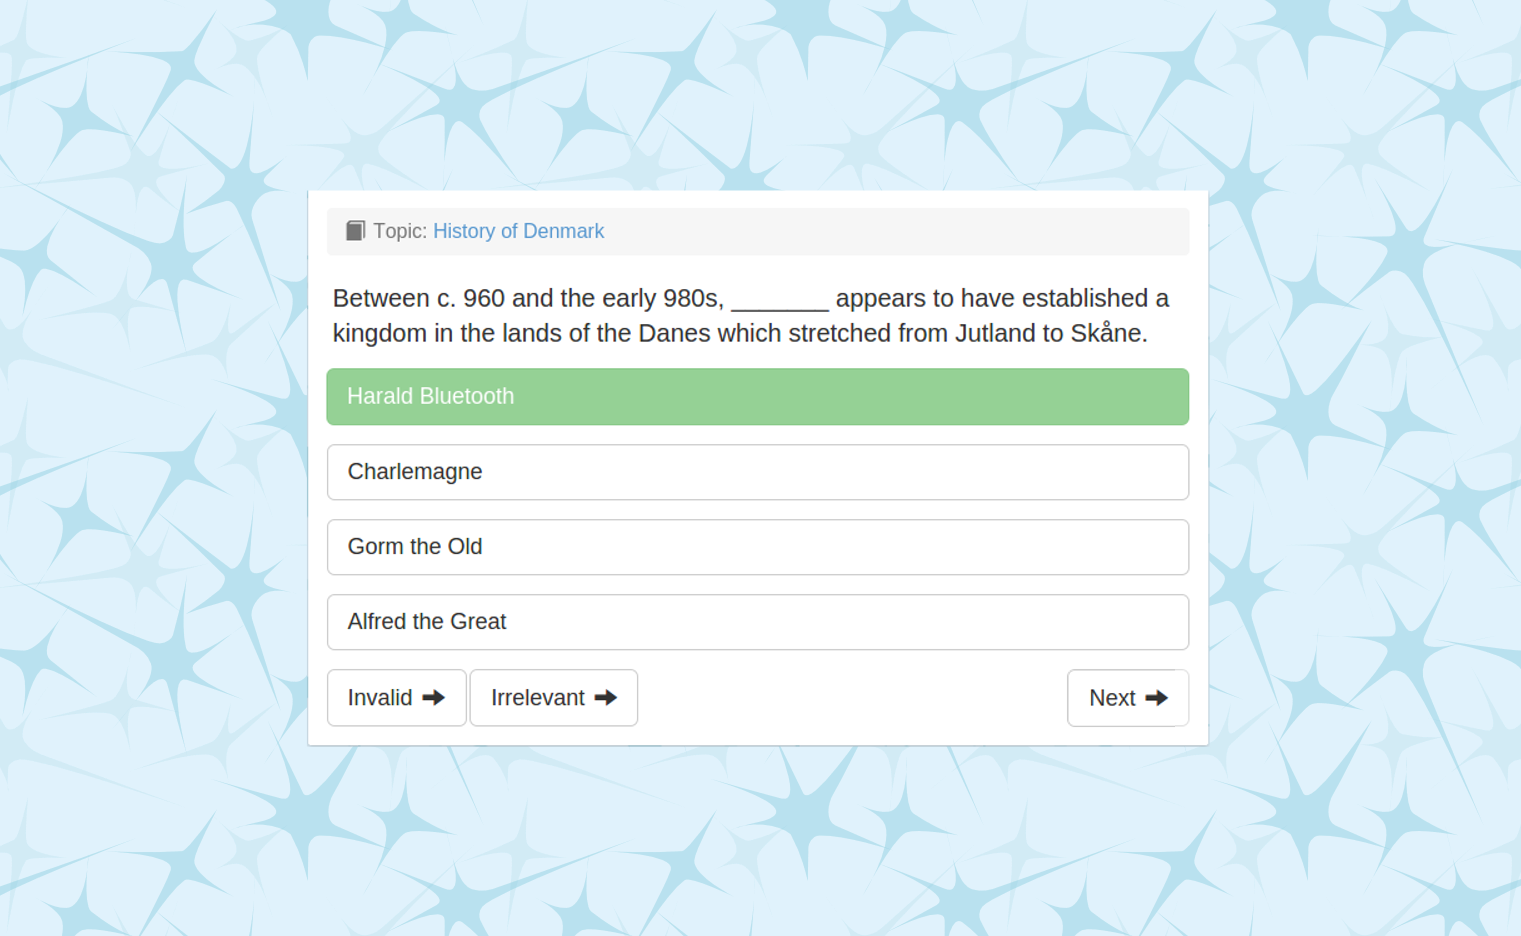
\includegraphics[scale=0.3]{img/question-answered2.png}}
\begin{frame}[plain]
\end{frame}
}
% ------------------------------------------------------------------------------
% --------------------------- SLIDE --------------------------------------------
\begin{frame}
\frametitle{Architektura}
\makebox[\textwidth][c]{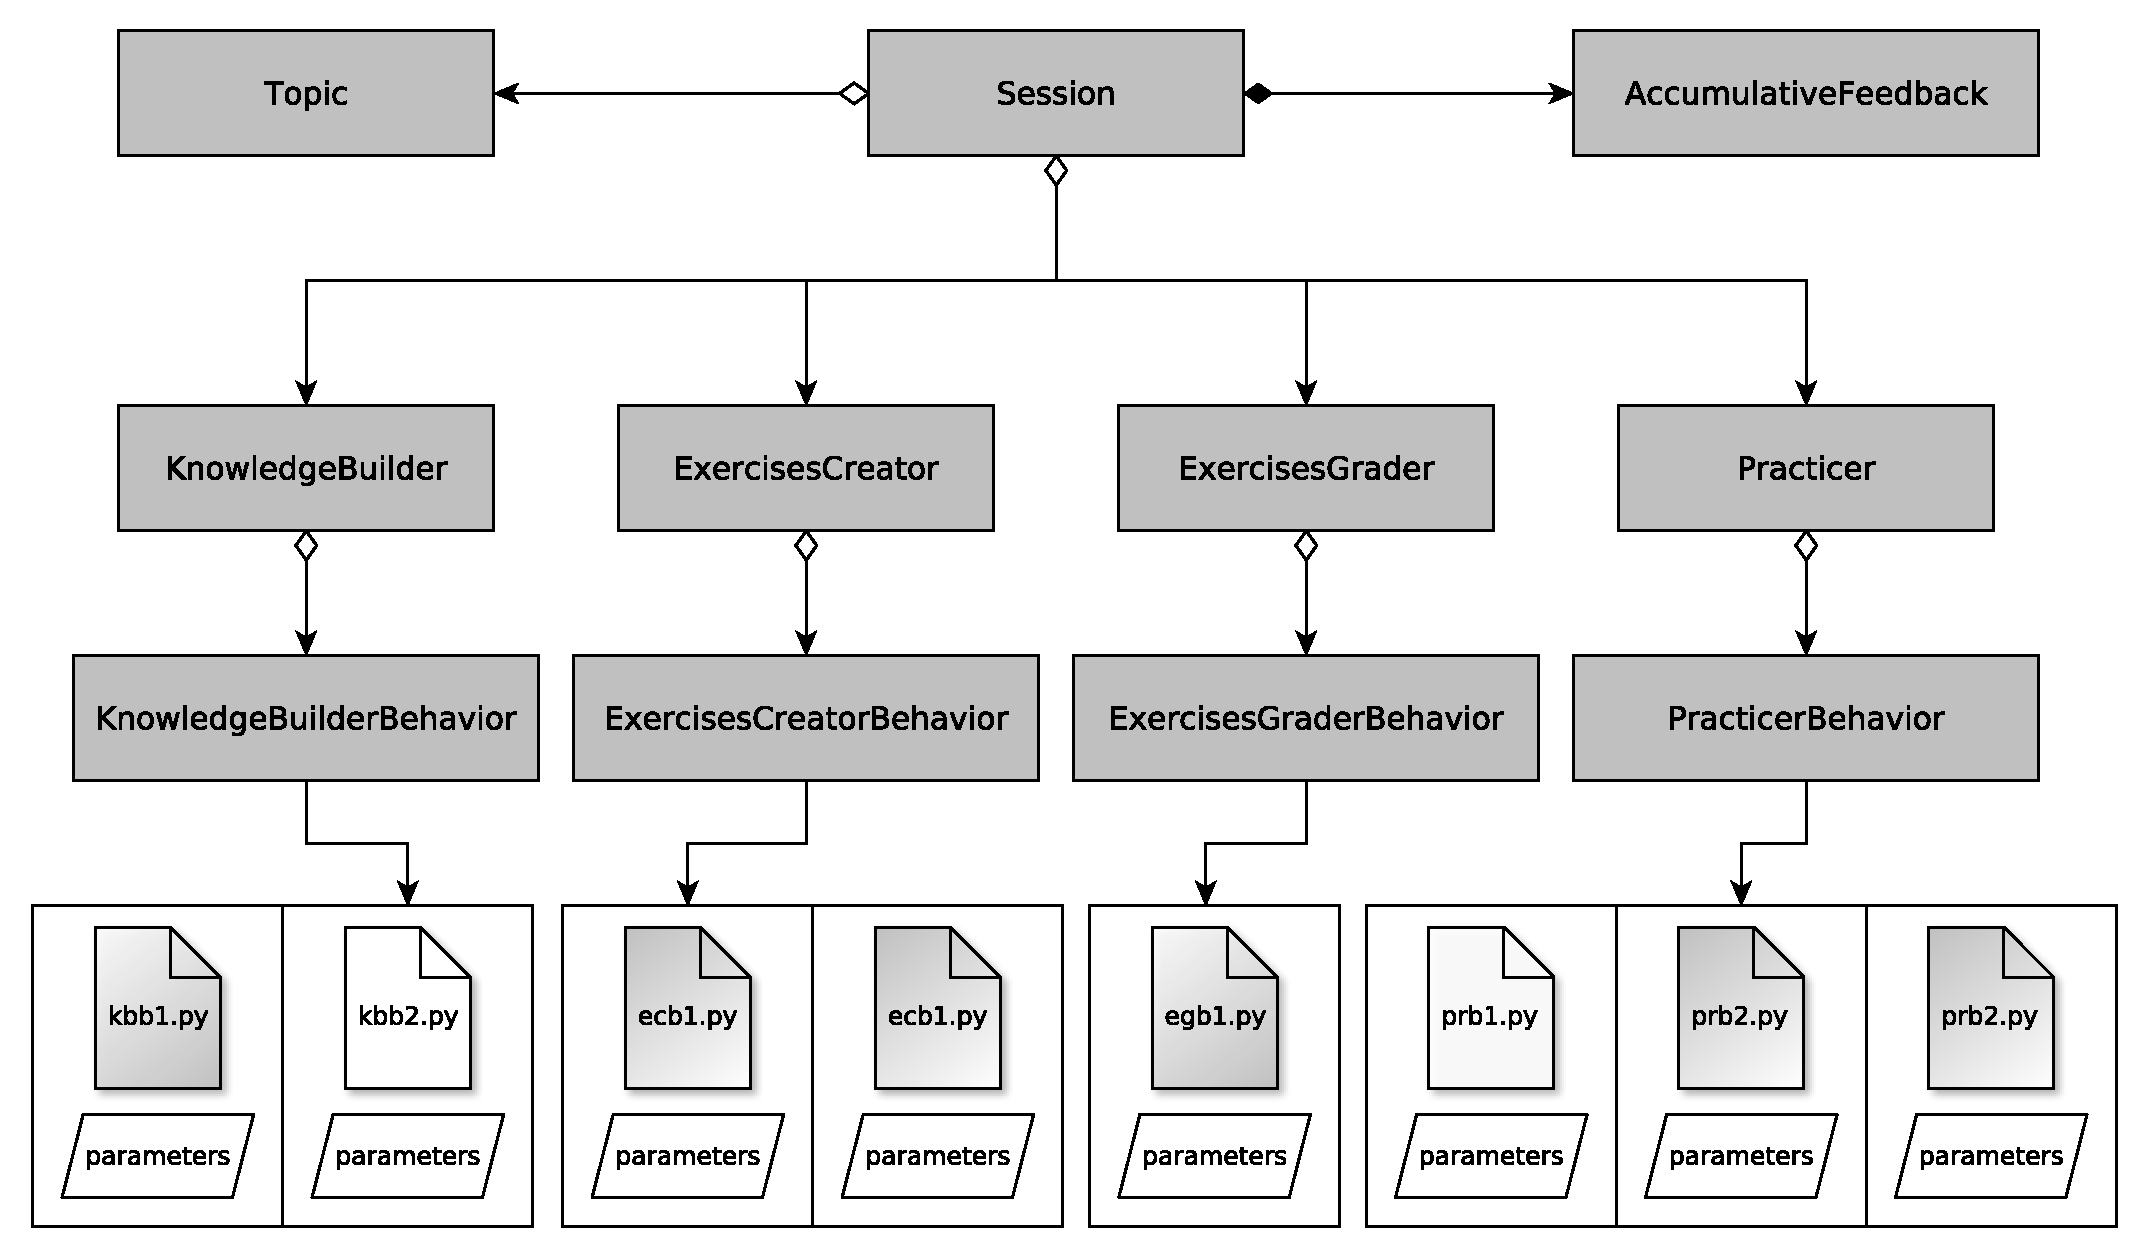
\includegraphics[width=1.15\textwidth]{../images/architecture.pdf}}
\end{frame}
% ------------------------------------------------------------------------------
% --------------------------- SLIDE --------------------------------------------
\begin{frame}
\frametitle{Tok dat}
\makebox[\textwidth][c]{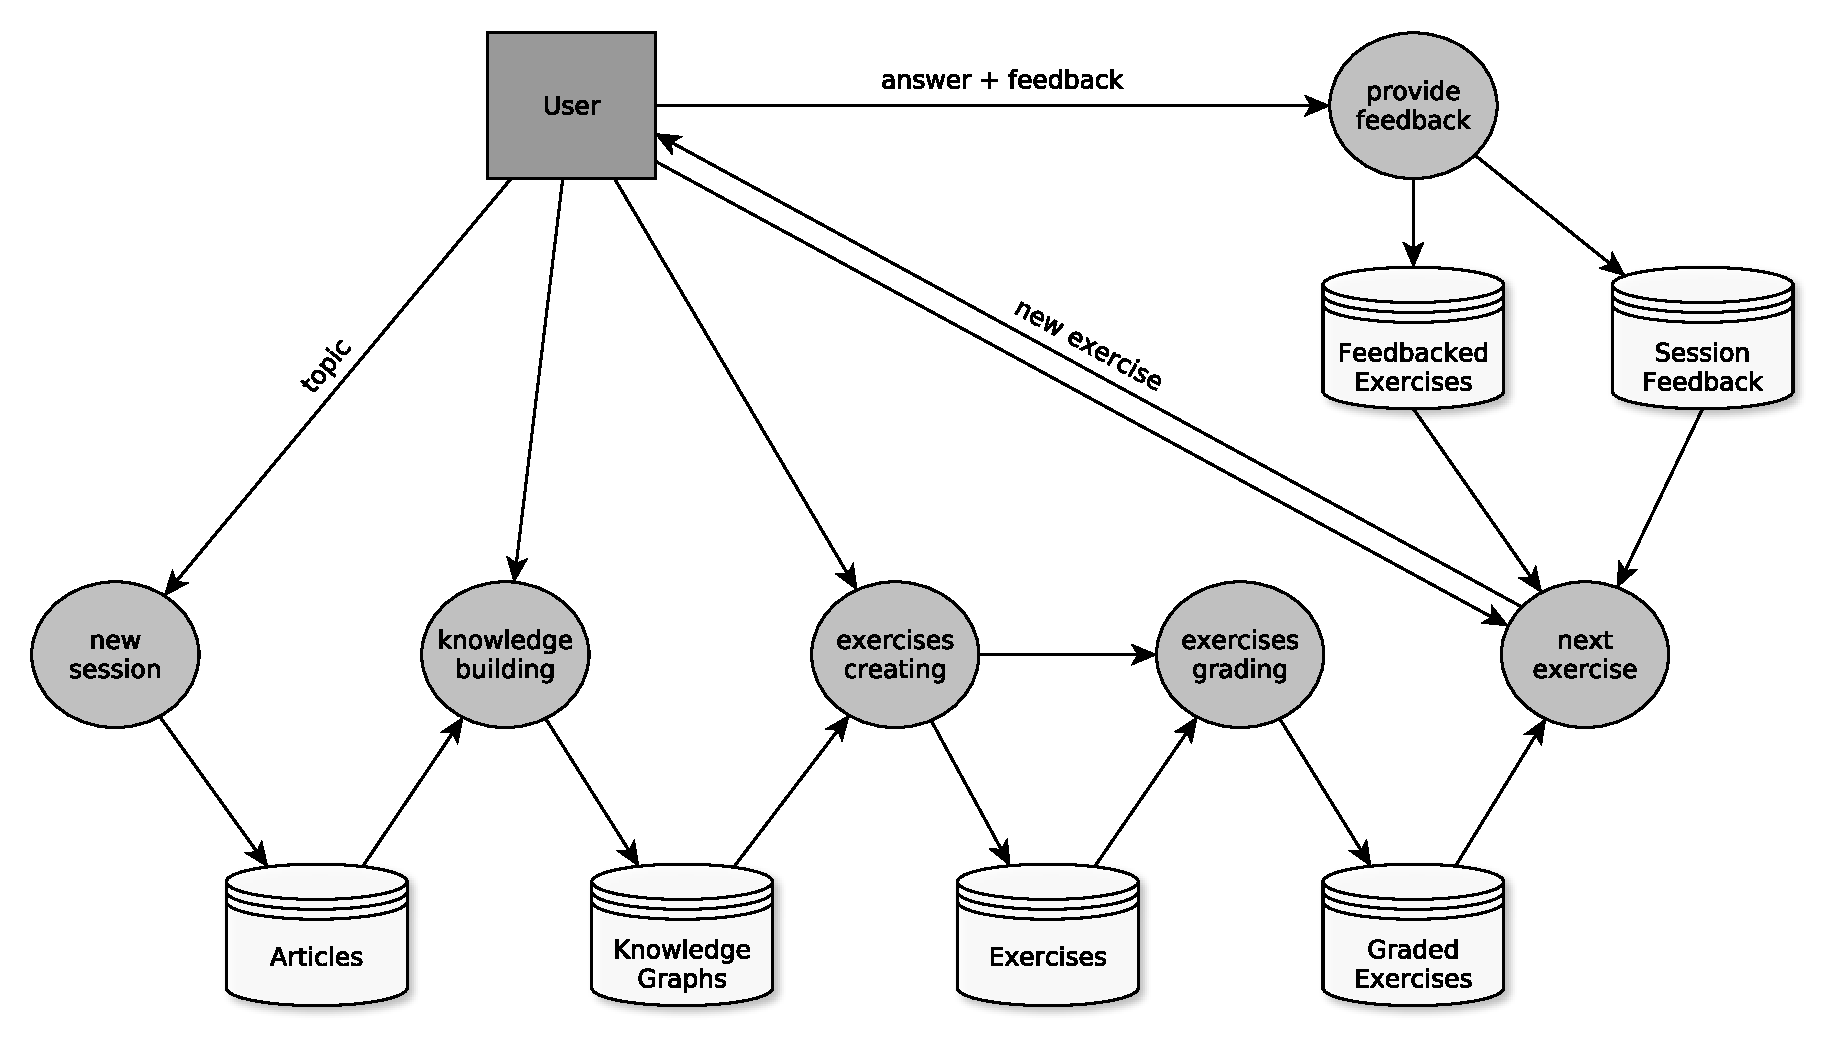
\includegraphics[width=1.15\textwidth]{../images/data-flow-diagram.pdf}}
\end{frame}
% ------------------------------------------------------------------------------
% --------------------------- SLIDE --------------------------------------------
\begin{frame}
\frametitle{Extrakce znalostí}
\begin{itemize}
\item stažení článku z Wikipedie
\item shallow parsing (tokenizace a tagování)
\item odvození výskytů pojmů
\item zjištění typů všech pojmů (DBpedie)
\item filtrování vět
\item uložení informace o pojmu ve větě
\end{itemize}
\end{frame}
% ------------------------------------------------------------------------------
% --------------------------- SLIDE --------------------------------------------
\begin{frame}
\frametitle{Pojem ve větě}
\makebox[\textwidth][c]{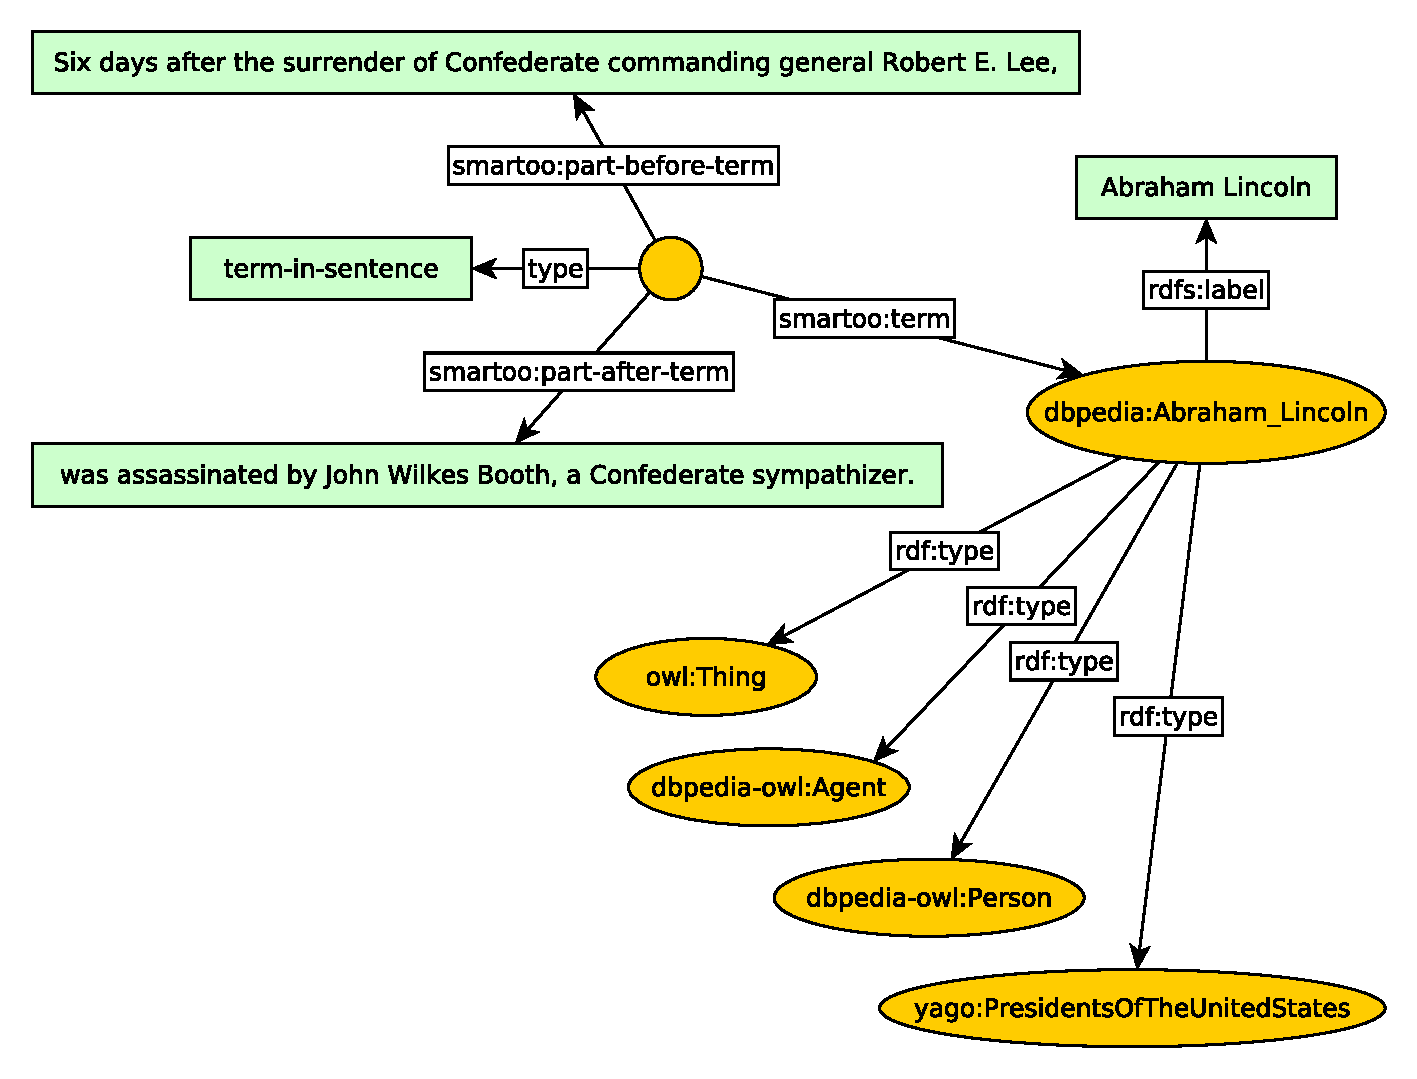
\includegraphics[width=1.15\textwidth]{../images/quasi-fact-lincoln.pdf}}
\end{frame}
% ------------------------------------------------------------------------------
% --------------------------- SLIDE --------------------------------------------
\begin{frame}
\frametitle{Generování otázek}
\begin{itemize}
\item ... NOTE: cilem neni seznamit se systemem! (strucnost!)
\end{itemize}
\end{frame}
% ------------------------------------------------------------------------------
% --------------------------- SLIDE --------------------------------------------
\begin{frame}
\frametitle{Hodnocení otázek}
\begin{itemize}
\item ...
\end{itemize}
\end{frame}
% ------------------------------------------------------------------------------
% --------------------------- SLIDE --------------------------------------------
\begin{frame}
\frametitle{Adaptabilní procvičování}
\begin{itemize}
\item ...
\end{itemize}
\end{frame}
% ------------------------------------------------------------------------------
% --------------------------- SLIDE --------------------------------------------
\begin{frame}
\frametitle{Evaluace}
\begin{itemize}
\item 71 procvičování
\item 616 otázek
\item průměrná úspěšnost 72 \%
\end{itemize}
\end{frame}
% ------------------------------------------------------------------------------
% --------------------------- SLIDE --------------------------------------------
\begin{frame}
\frametitle{Hodnocení otázek}
\begin{center}

\begin{tikzpicture}
\pie [color={lightBlue, myYellow, lightRed}] {91.7/ok , 5.5/irrelevant , 2.8/invalid}
\end{tikzpicture}

\end{center}
\end{frame}
% ------------------------------------------------------------------------------
% --------------------------- SLIDE --------------------------------------------
\begin{frame}
\frametitle{Závěrečné hodnocení}
\begin{center}

\begin{tikzpicture}   %[nodes = {font=\sffamily}]
\pie [color={lightGreen, lightBlue, lightRed}] {31/good , 65/so so , 4/bad}
\end{tikzpicture}

\end{center}
\end{frame}
% ------------------------------------------------------------------------------
% --------------------------- SLIDE --------------------------------------------
\begin{frame}[plain]
\begin{center}
Děkuji za pozornost.
\end{center}
\end{frame}
% ------------------------------------------------------------------------------

\end{document}
